\chapter{Результаты}\label{ch:results}

Подробные результаты работы модуля алгебраической декомпозиции представлены на рисунке \ref{fig:time_res}, где сравнивается работа модуля без повторной попытки решения с работой решателя без модуля алгебраической декомпозиции. Суммарное ускорение времени решения при включении алгебраической декомпозиции составило:
\begin{itemize}
    \item 
        с повторной попыткой решения: 77\% 
    \item
        без повторной попытки: 81\% 
\end{itemize}

\begin{figure}[h]
	\centering
	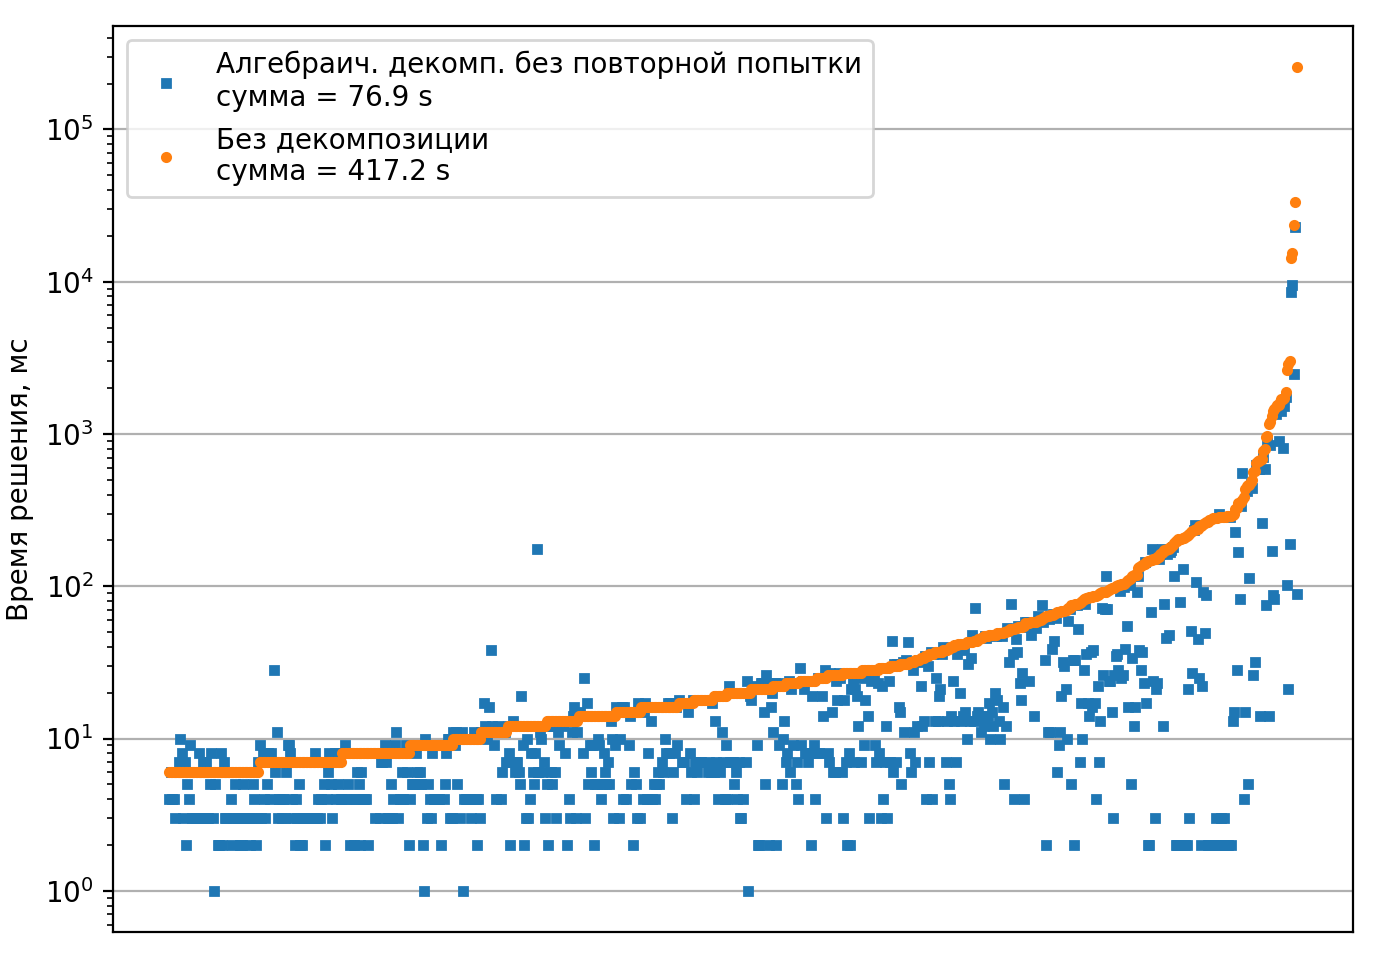
\includegraphics[width=0.6\linewidth]{figures/fig_time_results.png}
	\caption{Результаты работы модуля алгебраической декомпозиции в 3D на индустриальной тестовой базе из ~3000 тестов}
	\label{fig:time_res}
\end{figure}

Процент решенных тестов составил:
\begin{itemize}
    \item с повторной попыткой решения:  95.6\% $\rightarrow$ 97.6\%
    \item  без повторной попытки:  95.6\% $\rightarrow$ 96.7\%
\end{itemize}
